\documentclass[]{beamer}

\usetheme{Antibes}
\usecolortheme{beaver}
\usefonttheme{professionalfonts}
\setbeamercolor{block title}{bg=red!30,fg=black}

\usepackage{pgfpages}
\usepackage[italian]{babel} 
\usepackage[T1]{fontenc}
\usepackage[utf8x]{inputenc}
\usepackage{graphicx}
\usepackage{xcolor}
\usepackage{float}
\usepackage{subfig}
\usepackage[autoplay]{animate}
\usepackage{tikz}
\usepackage{pgfplots}
\usepackage{tikz-3dplot}
\usepackage[mode=image|tex]{standalone}

% New operators
\DeclareMathOperator*{\atan2}{atan2}            % Atan2 
\DeclareMathOperator*{\asin}{asin}              % Asin
\DeclareMathOperator*{\sgn}{sgn}                % Sgn
\DeclareMathOperator*{\diag}{diag}              % Diag
\DeclareMathOperator*{\subjectto}{subject\hspace{2pt}to}

\setbeamercovered{dynamic}

\pgfdeclareimage[height=1cm]{logo_unipd}{images/unipd}
\pgfdeclareimage[height=2cm]{logo_dei}{images/dei}
%\logo{\pgfuseimage{logo_unipd}}
\titlegraphic{\pgfuseimage{logo_dei}}

\title[]{Model identification and flight control design for the Prometheus mapping drone}
\author[Nicola Dal Lago]{ Nicola Dal Lago}
\date[10 ottobre 2016]{10 ottobre 2016}
\institute[DEI Unipd]{Corso di Laurea Magistrale in Ingegneria dell'Automazione\\ Dipartimento di Ingegneria dell'Informazione}

\begin{document}
\frame{\titlepage}


	\section{Introduzione}
	
	\begin{frame}{Prometheus mapping drone}
		\centering	
		\begin{columns}
			\begin{column}{.5\textwidth}
				\centering
				\begin{figure}
					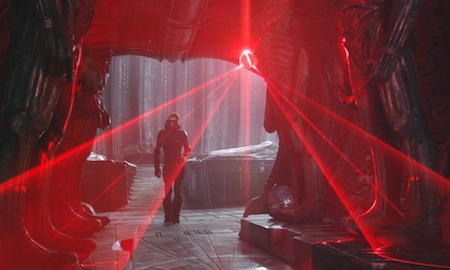
\includegraphics[scale=0.31]{images/prometheus_film.jpg}
				\end{figure}
			\end{column}
			\begin{column}{.5\textwidth}
				\centering
				\begin{block}{Scopo del progetto}
					Realizzazione di un UAV per navigazione e mappatura 3D in autonomo
				\end{block}
			\end{column}
		\end{columns}
		\centering
		\begin{block}{Contributo di questa tesi:}
			\begin{itemize}
				\item[1] Modello matematico
				\item[2] Identificazione di sistema 
				\item[3] Generatore di traiettorie
				\item[4] Algoritmo di controllo
			\end{itemize}
		\end{block}
	\end{frame}
	
	\begin{frame}{Design}
		\centering
		\begin{columns}
			\begin{column}{.5\textwidth}
				\centering
				\begin{figure}
					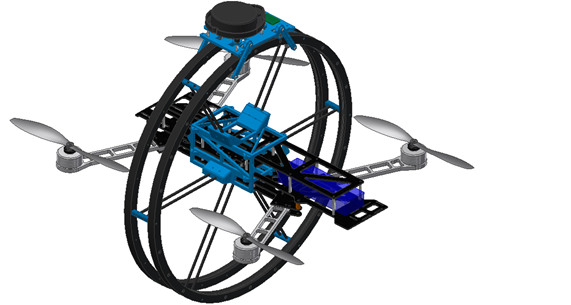
\includegraphics[scale=0.35]{images/render1.png}
				\end{figure}
			\end{column}
			\begin{column}{.5\textwidth}
				\centering
				\begin{itemize}
					\item Telaio di un quadricottero standard 
					\item Uso di un sensore laser Lidar, mapping in 2D
					\item Aggiunta di una piattaforma rotante per mapping in 3D
				\end{itemize}
			\end{column}
		\end{columns}
	\end{frame}
	
	
	\section{Modello matematico}
	
	\begin{frame}{Modello matematico}
		\centering
		Cinematica di Newton-Eulero
		\begin{equation*}
			\begin{bmatrix}
				m \cdot I_{3} & \mathbf{0} \\
				\mathbf{0}^T          & I_{cm}
			\end{bmatrix}
			\begin{bmatrix}
				\mathbf{\ddot{x}_B}         \\
				\boldsymbol{\dot{\omega}_B}
			\end{bmatrix}
			+
			\begin{bmatrix}
				\mathbf{0}                                                      \\
				\boldsymbol{\omega_B} \times I_{cm} \cdot \boldsymbol{\omega_B}
			\end{bmatrix}
			=
			\begin{bmatrix}
				\mathbf{f}        \\
				\boldsymbol{\tau}
			\end{bmatrix}
		\end{equation*}
		\begin{columns}
			\begin{column}{.55\textwidth}
				\centering
				\begin{figure}
					\includestandalone[scale=0.5]{standalone/quadrotor}
				\end{figure}
			\end{column}
			\begin{column}{.55\textwidth}
				\centering
				\small
				\begin{align*}
					\mathbf{f}_i(t) &= a_{f,i}\Omega_i^2\mathbf{n}_i = a_{f,i}\Omega_{max, i}^2 u_i(t)^2\mathbf{n}_i \\
					\boldsymbol{\tau}_i(t) &= -\sgn(\Omega_i)b_{f,i}\Omega_{max,i}^2u_i(t)^2\mathbf{n}_i \\
					u_i(t) &\approx \frac{1}{\tau_i s+1}u_{in,i}(t)
				\end{align*}
				\begin{equation*}
					\begin{bmatrix}
						\mathbf{f}_{total} \\
						\boldsymbol{\tau}_{total}
					\end{bmatrix}
					=
					\begin{bmatrix}
						\sum\limits_{i=1}^{4} \mathbf{f}_i(u_i^2) \\
						\sum\limits_{i=1}^{4} \mathbf{l}_i \times \mathbf{f}_i(u_i^2) + \boldsymbol{\tau}_i(u_i^2)
					\end{bmatrix}
				\end{equation*}
			\end{column}
		\end{columns}
	\end{frame}
	
	\begin{frame}
		\centering
		\begin{columns}
			\begin{column}{.4\textwidth}
				\centering
				\begin{figure}
					\includestandalone[scale=0.55]{standalone/quadrotor_cart2}
				\end{figure}					
			\end{column}
			\begin{column}{.4\textwidth}
				\centering
				\begin{figure}
					\includestandalone[scale=0.55]{standalone/quadrotor_cart}
				\end{figure}					
			\end{column}
		\end{columns}
		\begin{block}{Dinamica complessiva}
			\setlength\abovedisplayskip{0pt}
			\tiny
			\begin{equation*}
			\begin{split}
				\begin{bmatrix}
					\ddot{\mathbf{x}}_B \\
					\dot{\boldsymbol{\omega}}_B
				\end{bmatrix}
				&=
				\begin{bmatrix}
					\dots & \frac{a_{f,i}\Omega_{max,i}^2\mathbf{n}_i}{m} & \dots \\
					\dots & \textcolor{blue}{I_{cm}^{-1}}\Big[ (\textcolor{blue}{\mathbf{l}_i}+\boldsymbol{\Delta l})\times a_{f,i}\Omega^2_{max,i}\mathbf{n}_i-\sgn(\Omega_i)b_{f,i}\Omega_{max,i}^2\mathbf{n}_i\Big] & \dots
				\end{bmatrix}
				\begin{bmatrix}
					\vdots \\
					u_i^2 \\
					\vdots
				\end{bmatrix}
					+ \\
					&+
				\begin{bmatrix}
					\mathbf{0} \\
					\textcolor{blue}{I_{cm}^{-1}}\bigl(\boldsymbol{\omega}_B \times I_{cm} \boldsymbol{\omega}_B \bigl)
				\end{bmatrix}
				+
				\textcolor{blue}{
				\frac{1}{m_{cart}}
				\begin{bmatrix}
					\mathbf{f}_{cart} \\
					\mathbf{0}
				\end{bmatrix} 
				}
			\end{split}
			\end{equation*}
		\end{block}
	\end{frame}


	\section{Identificazione di sistema}
	
	\begin{frame}{Identificazione del sistema con filtrto di Kalman esteso}
		\centering
		\begin{columns}
			\begin{column}{.4\textwidth}
				\centering
				\begin{block}{Semplificazioni}
					\setlength\abovedisplayskip{-10pt}
					\begin{align*}
						a_{f,i}\Omega_{max,i}^2 &\approx a_f \\
						b_{f,i}\Omega_{max,i}^2 &\approx b_f \\
						\tau_i &\approx \tau
					\end{align*}
				\end{block}
			\end{column}
			\begin{column}{.6\textwidth}
				\centering
				\begin{block}{Linearizzazione}
					\begin{itemize}
						\item $I_{cm}^{-1}\bigl(\boldsymbol{\omega}_B \times I_{cm} \boldsymbol{\omega}_B \bigl) \approx 0$
						\item muovere il quadrato degli ingressi al modello del motore
					\end{itemize}
				\end{block}
			\end{column}
		\end{columns}
		\centering
		Definisco nuovo stato aumentato
		\tiny
		\begin{equation*}
			\mathbf{x}_{est}=
			\begin{bmatrix}
				\boldsymbol{\omega}_B & \mathbf{u}_{in} & \boldsymbol{\beta} & \tau
			\end{bmatrix}^T
			\in \rm I\!R^{15}, \quad \boldsymbol{\beta}=
			\begin{bmatrix}
				\frac{a_f}{m} & \frac{a_f}{I_{xx}} & \frac{a_f}{I_{yy}} & \frac{a_f}{I_{zz}} & \frac{b_f}{I_{zz}} & \Delta l_x & \Delta l_y 
			\end{bmatrix}^T
		\end{equation*}
		\normalsize
		e aggiungo dinamica dei parametri
		\begin{gather*}
			\boldsymbol{\omega}_{k+1} = \boldsymbol{\omega}_k \qquad \tau_{k+1} = \tau_{k} \\
			\Downarrow \\
			\text{Filtro di Kalman esteso}
		\end{gather*}
	\end{frame}
	
	\begin{frame}{Risultati sperimentali}
		\centering
		\begin{columns}
			\begin{column}{.5\textwidth}
				\centering
				\begin{figure}
					\includestandalone[scale=0.8]{plots/identification}
				\end{figure}
			\end{column}
			\begin{column}{.5\textwidth}
				\centering
				\begin{itemize}
					\item Carrello non in movimento
					\item Identificazione dei parametri anche con condizioni iniziali molto sbagliate
				\end{itemize}
			\end{column}
		\end{columns}
	\end{frame}
	
	
	\section{Generatore di traiettorie}
	
	
	\begin{frame}{Generatore di traiettorie}
		\centering 
		\begin{columns}
			\begin{column}{.4\textwidth}
				\centering
				Minimizzare funzione costo
				\begin{alignat}{2}
					\min\qquad & \mathbf{c}^TH\mathbf{c} + f^T\mathbf{c} \nonumber \\
					\subjectto \qquad & A\mathbf{c} \le \mathbf{b} \nonumber \\
					& A_{eq}\mathbf{c} = \mathbf{b}_{eq} \nonumber
				\end{alignat}
			\end{column}
			\begin{column}{.1\textwidth}
				\centering
				\begin{equation*}
					\Rightarrow
				\end{equation*}
			\end{column}
			\begin{column}{.5\textwidth}
				\centering
				\begin{itemize}
					\item Problema quadratico di programmazione matematica 
					\item Vincoli nei waypoints iniziali e finali
					\item Vincoli di sicurezza
				\end{itemize}
			\end{column}
		\end{columns}
		\begin{figure}
			\includestandalone[scale=0.45]{plots/trajectory}
		\end{figure}
	\end{frame}

	
	\section{Controllo}
	
	\begin{frame}{Controllo}
		\centering
		\begin{columns}
			\begin{column}{.45\textwidth}
				\setlength\abovedisplayskip{-10pt}
				\centering
				\begin{block}{Definizione degli errori}
					\begin{align*}
						\mathbf{e}_x &= \mathbf{x} - \mathbf{x}_d \\ 
						\mathbf{e}_v &= \dot{\mathbf{x}} - \dot{\mathbf{x}}_d \\
						\mathbf{e}_R &= \frac{1}{2}\bigl(R_c^TR-R^TR_C \bigl)^{\vee} \\
						\mathbf{e}_{\omega} &= \boldsymbol{\omega} - R^TR_C\hat{\boldsymbol{\omega}}_c
					\end{align*}
					$R_C$ è tale che $R_C \in SO(3)$
				\end{block}
			\end{column}
			\begin{column}{.55\textwidth}
				\centering
				\begin{block}{Contributo di forza}
					\setlength\abovedisplayskip{-10pt}
					\begin{equation*}
						f = -(k_x\mathbf{e}_x+k_v\mathbf{e}_v-g\mathbf{e}_3-\ddot{\mathbf{x}}_d)^TR\mathbf{e}_3
					\end{equation*}
				\end{block}
				\begin{block}{Contributo di momento torcente}
					\setlength\abovedisplayskip{-10pt}
					\begin{equation*}
						\boldsymbol{\tau} = -k_R\mathbf{e}_R - k_{\omega}\boldsymbol{e}_{\omega} + \boldsymbol{\omega}\times I_{cm}\boldsymbol{\omega}
					\end{equation*}
				\end{block}
			\end{column}
		\end{columns}
		\begin{figure}
			\includestandalone[scale=0.65]{standalone/controller}
		\end{figure}
	\end{frame}
	
	\begin{frame}{Risultati in simulazione}
		\centering
		\begin{figure}
			\includestandalone[scale=0.65]{plots/control}
		\end{figure}
	\end{frame}
	
	
	\section{Conclusioni e sviluppi futuri}
		
	\begin{frame}{Conclusioni e sviluppi futuri}
		\centering
		\begin{block}{Conclusioni}
			\begin{itemize}
				\item Identificazione del modello semplificato con filtro di Kalman 
				\item Generatore di traiettorie lisce
				\item Controllo con compensazione del movimento del sensore
			\end{itemize}
		\end{block}
		\begin{block}{Sviluppi futuri}
			\begin{itemize}
				\item Identificazione per il modello non lineare
				\item Imporre vincoli basati sulla dinamica dell'UAV nelle traiettorie
				\item Controllo in grado di prevedere la dinamica, come MPC
			\end{itemize}
		\end{block}
	\end{frame}
	
	
	\section{}
	
	\begin{frame}
		\centering
		\Huge
		\textbf{\textcolor{red}{Grazie per l'attenzione!}}
	\end{frame}
	
	
	\section{Appendici}
	
	\begin{frame}{Prometheus mapping drone}
		\centering
		\begin{columns}
			\begin{column}{.5\textwidth}
				\centering
				\begin{figure}
					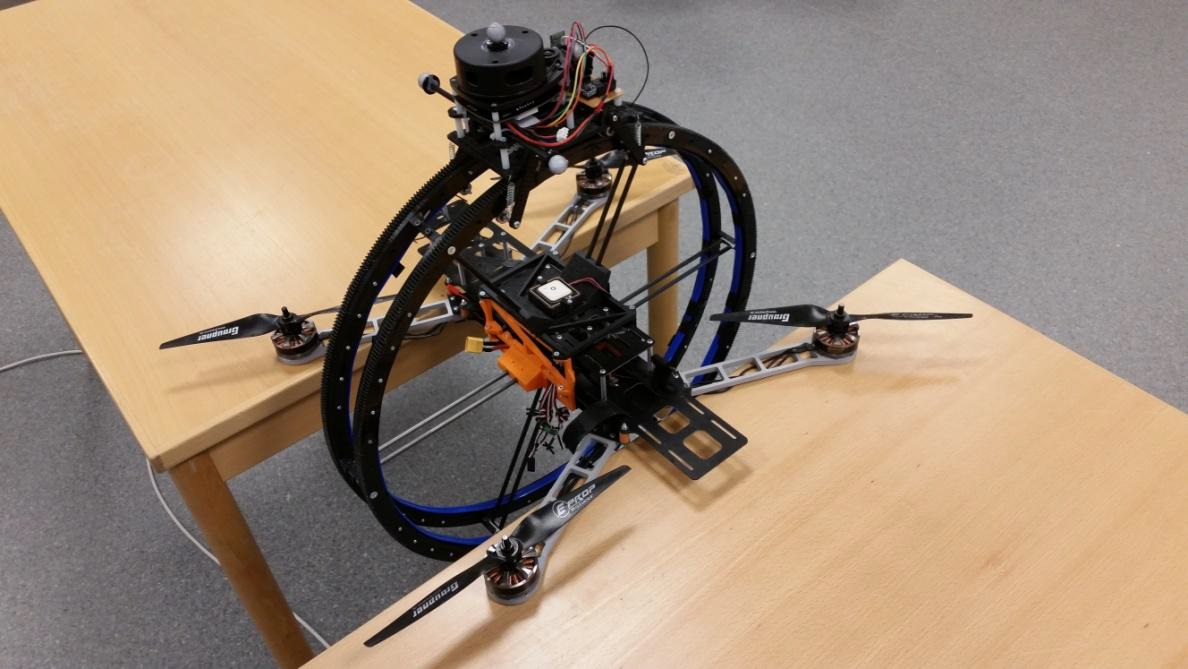
\includegraphics[scale=0.17]{images/prometheus1.jpg} \\
					\vspace{5pt}
					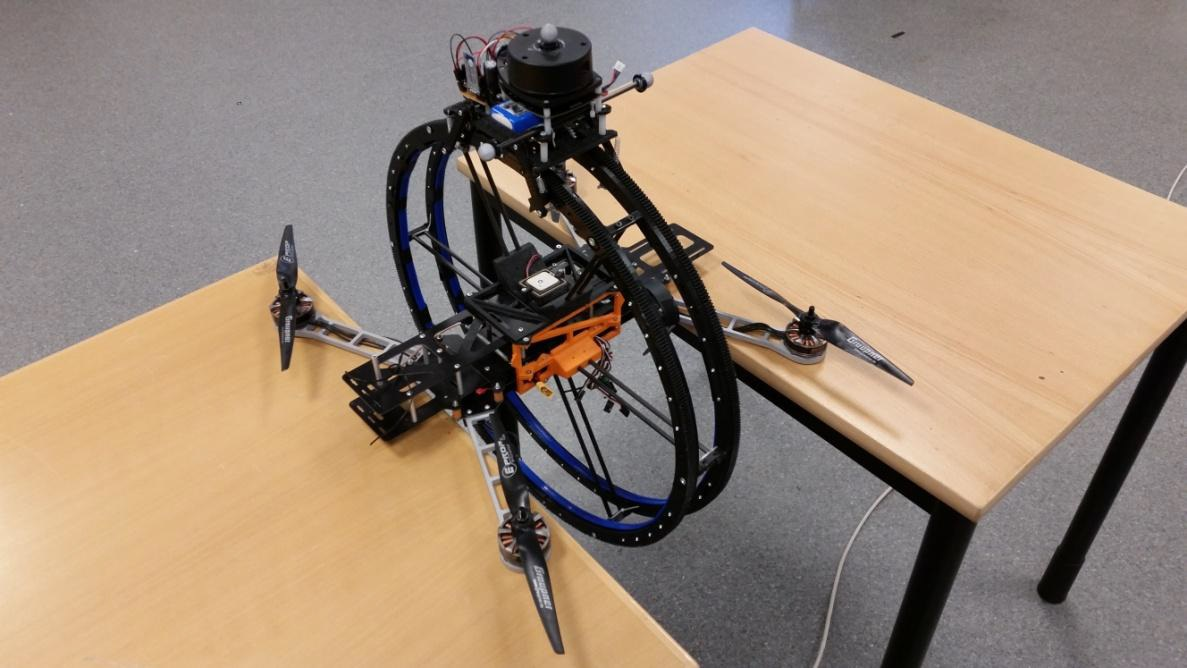
\includegraphics[scale=0.17]{images/prometheus2.jpg}
				\end{figure}
			\end{column}
			\begin{column}{.5\textwidth}
				\centering
				\begin{figure}
					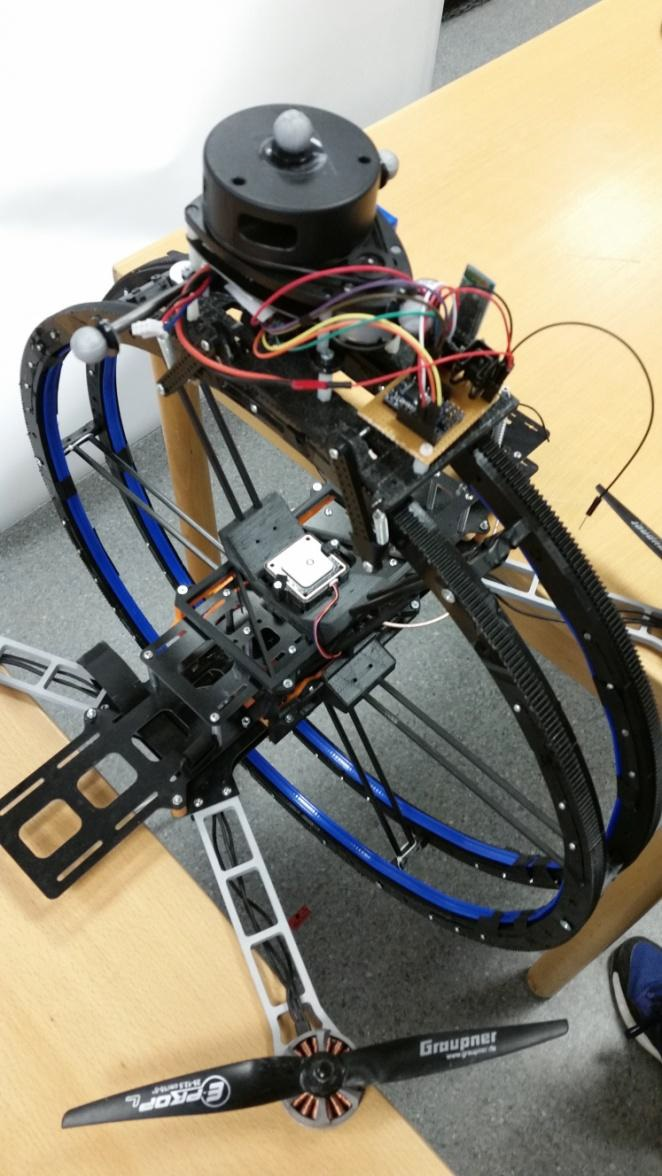
\includegraphics[scale=0.2]{images/prometheus3.jpg}
				\end{figure}
			\end{column}
		\end{columns}
	\end{frame}
	
	\begin{frame}{Model Predictive Control (MPC)}
		\centering
		\begin{block}{Definizione}
			\setlength\abovedisplayskip{-10pt}
			\begin{align}
				&\min_{U_{t\to t+N|t}} &&J_t=\sum_{i=1}^N||\mathbf{r}_i-\mathbf{x}_i||^2_{W_x} + \sum_{i=1}^N||\boldsymbol{\Delta}\mathbf{u}||^2_{W_u} \label{eq:MPC} \nonumber \\
				&\subjectto &&\mathbf{x}_{t+k+1|t}=A\mathbf{x}_{t+k|t}+B\mathbf{u}_{t+k|t}, \quad & k=1,\dots,N \nonumber \\
				& &&\mathbf{x}_{t+k|t} \in X, \quad \mathbf{u}_{t+k|t} \in U, \quad & k=1,\dots,N \nonumber \\
				& &&\mathbf{x}_{t|t}=\mathbf{x}(t) \nonumber
			\end{align}
		\end{block}
		\begin{columns}
			\begin{column}{.5\textwidth}
				\centering
				Pro:
				\begin{itemize}
					\item Include modello motori
					\item Vincoli negli ingressi
				\end{itemize}
			\end{column}
			\begin{column}{.5\textwidth}
				\centering
				Contro:
				\begin{itemize}
					\item Linearizzazione del modello
					\item Complessità computazionale
				\end{itemize}
			\end{column}
		\end{columns}
	\end{frame}
	
	\begin{frame}
		\centering Modello lineare più approsimazione piccoli angoli 
		\begin{block}{Switching MPC}
			\begin{figure}
				\includestandalone[scale=0.65]{standalone/switchingMPC}
			\end{figure}
		\end{block}
	\end{frame}
	
\end{document}